
\documentclass[12pt,a4paper]{article}

\usepackage[a4paper,margin=1in]{geometry}
\usepackage{graphicx}
\usepackage{booktabs}
\usepackage{amsmath,amssymb}
\usepackage{float}
\usepackage{hyperref}
\usepackage{xcolor}
\usepackage{listings}
\usepackage{enumitem}
\usepackage{fancyhdr}
\usepackage{longtable}
\usepackage{array}
\usepackage{caption}

\hypersetup{
    colorlinks=true,
    linkcolor=blue,
    urlcolor=blue
}

\pagestyle{fancy}
\fancyhf{}
\lhead{ICS1512}
\rhead{Machine Learning Algorithms Laboratory}
\cfoot{\thepage}

\lstset{
    language=Python,
    basicstyle=\ttfamily\small,
    numbers=left,
    frame=single,
    breaklines=true,
    showstringspaces=false,
    columns=fullflexible
}

\setlength{\parindent}{0pt}
\setlength{\parskip}{6pt}

\begin{document}

% ============================================================
% TITLE / EXPERIMENT INFORMATION
% ============================================================

\begin{tabular}{|p{4cm}|p{11cm}|}
\hline
Experiment No. & 3 \\ \hline
Experiment Title & Regression Analysis using Linear Regression and Regularized Regression Models \\ \hline
GitHub Repository & \url{https://github.com/HarshitaaB-2606} \\ \hline
Student Name & \textit{Harshitaa B} \\ \hline
Register Number & \textit{3122247001021} \\ \hline
Faculty & Dr. Poreddy Ajay Kumar Reddy \\ \hline
Submission Date & \textit{16th August 2026} \\ \hline
\end{tabular}

\vspace{0.5cm}

\begin{center}
    {\Large\textbf{ICS1512 -- Machine Learning Algorithms Laboratory}}\\[0.2cm]
    {\large\textbf{Experiment 3: Regression Analysis}}
\end{center}

% ============================================================
\section{Objective}
% ============================================================

The objectives of this experiment are:

\begin{enumerate}[label=\arabic*.]
    \item To implement Linear Regression for predicting a continuous target variable.
    \item To implement Ridge, Lasso, and Elastic Net Regression using regularization techniques.
    \item To preprocess a dataset containing numerical and categorical attributes by handling missing values, encoding categorical variables, and scaling numerical variables.
    \item To use five-fold cross-validation for model evaluation and Grid Search for hyperparameter selection.
    \item To compare Linear Regression, Ridge Regression, Lasso Regression, and Elastic Net Regression using Mean Absolute Error (MAE), Mean Squared Error (MSE), Root Mean Squared Error (RMSE), and $R^2$ score.
    \item To analyze the effect of regularization on model complexity, generalization, and regression coefficients.
    \item To study the feature-sparsity effect of Lasso Regression and compare the coefficients produced by the different models.
    \item To analyze possible overfitting and underfitting through training and test errors and to discuss the bias--variance trade-off.
    \item To identify the best-performing regression model for predicting the sanctioned loan amount.
\end{enumerate}

% ============================================================
\section{Problem Statement}
% ============================================================

The objective of this experiment is to predict the sanctioned loan amount using applicant-related information. The dataset contains a mixture of numerical and categorical attributes describing the applicant and loan application.

The input consists of applicant and loan-related features such as applicant income, co-applicant income, loan term, credit history, gender, marital status, number of dependents, education, self-employment status, and property area. The output is the continuous variable representing the sanctioned loan amount.

Four regression approaches are evaluated:

\begin{enumerate}
    \item Linear Regression
    \item Ridge Regression
    \item Lasso Regression
    \item Elastic Net Regression
\end{enumerate}

The provided dataset already contains separate training and testing files. Therefore, the supplied training set is used for model fitting, five-fold cross-validation, and hyperparameter tuning, while the supplied testing set is reserved for final evaluation.

The main objective is not only to obtain a low prediction error, but also to determine whether regularization improves generalization compared with ordinary Linear Regression.

% ============================================================
\section{Dataset Description}
% ============================================================

The experiment uses separate training and testing datasets. The target variable is the sanctioned loan amount.

\begin{longtable}{|p{6cm}|p{8cm}|}
\hline
\textbf{Dataset Property} & \textbf{Description} \\ \hline
Dataset Name & Loan-sanction regression dataset (training and testing CSV files) \\ \hline
Dataset Source & https://www.kaggle.com/datasets/altruistdelhite04/loan-prediction-problem-dataset \texttt{train.csv} and \texttt{test.csv} files. \\ \hline
Training Samples & 592 \\ \hline
Testing Samples & 362 \\ \hline
Target Variable & Loan amount sanctioned \\ \hline
Numerical Features & ApplicantIncome, CoapplicantIncome, Loan\_Amount\_Term, Credit\_History \\ \hline
Categorical Features & Loan\_ID, Gender, Married, Dependents, Education, Self\_Employed, Property\_Area \\ \hline
Number of Original Features & 11 \\ \hline
Transformed Features & 611 after preprocessing and one-hot encoding \\ \hline
Missing Values & Missing values were handled using imputation within the preprocessing pipeline. \\ \hline
Train-Test Split & A predefined train/test split was supplied as two separate CSV files; no additional random split was performed. \\ \hline
Target Type & Continuous numerical variable \\ \hline
\end{longtable}

\subsection{Feature Description}

\begin{longtable}{|p{4.5cm}|p{4cm}|p{5.5cm}|}
\hline
\textbf{Feature} & \textbf{Type} & \textbf{Description} \\ \hline
ApplicantIncome & Numerical & Income of the primary applicant. \\ \hline
CoapplicantIncome & Numerical & Income of the co-applicant. \\ \hline
Loan\_Amount\_Term & Numerical & Term/duration associated with the loan. \\ \hline
Credit\_History & Numerical & Credit-history indicator. \\ \hline
Loan\_ID & Categorical & Identifier associated with the loan application. \\ \hline
Gender & Categorical & Gender of the applicant. \\ \hline
Married & Categorical & Marital status of the applicant. \\ \hline
Dependents & Categorical & Number/category of dependents. \\ \hline
Education & Categorical & Education category of the applicant. \\ \hline
Self\_Employed & Categorical & Self-employment status. \\ \hline
Property\_Area & Categorical & Property-area category. \\ \hline
Loan Amount & Target & Continuous sanctioned loan amount to be predicted. \\ \hline
\end{longtable}

\textbf{Note:} The experiment results show that the preprocessing stage produced 611 transformed features. This is expected because categorical variables are converted into one-hot encoded representations.

% ============================================================
\section{Exploratory Data Analysis}
% ============================================================

Exploratory Data Analysis (EDA) was performed before model training to understand the structure and distribution of the data.

\subsection{Dataset Overview}

The training dataset contains 592 observations and the testing dataset contains 362 observations. The data contains both numerical and categorical variables. Since the target is continuous, this is a regression problem rather than a classification problem.

The numerical features identified during EDA were:

\begin{itemize}
    \item ApplicantIncome
    \item CoapplicantIncome
    \item Loan\_Amount\_Term
    \item Credit\_History
\end{itemize}

The categorical features identified were:

\begin{itemize}
    \item Loan\_ID
    \item Gender
    \item Married
    \item Dependents
    \item Education
    \item Self\_Employed
    \item Property\_Area
\end{itemize}

\subsection{Target Variable Distribution}

A histogram was used to inspect the distribution of the sanctioned loan amount.

\begin{figure}[H]
\centering
\IfFileExists{figs/Target_variable_distribution.png}{
    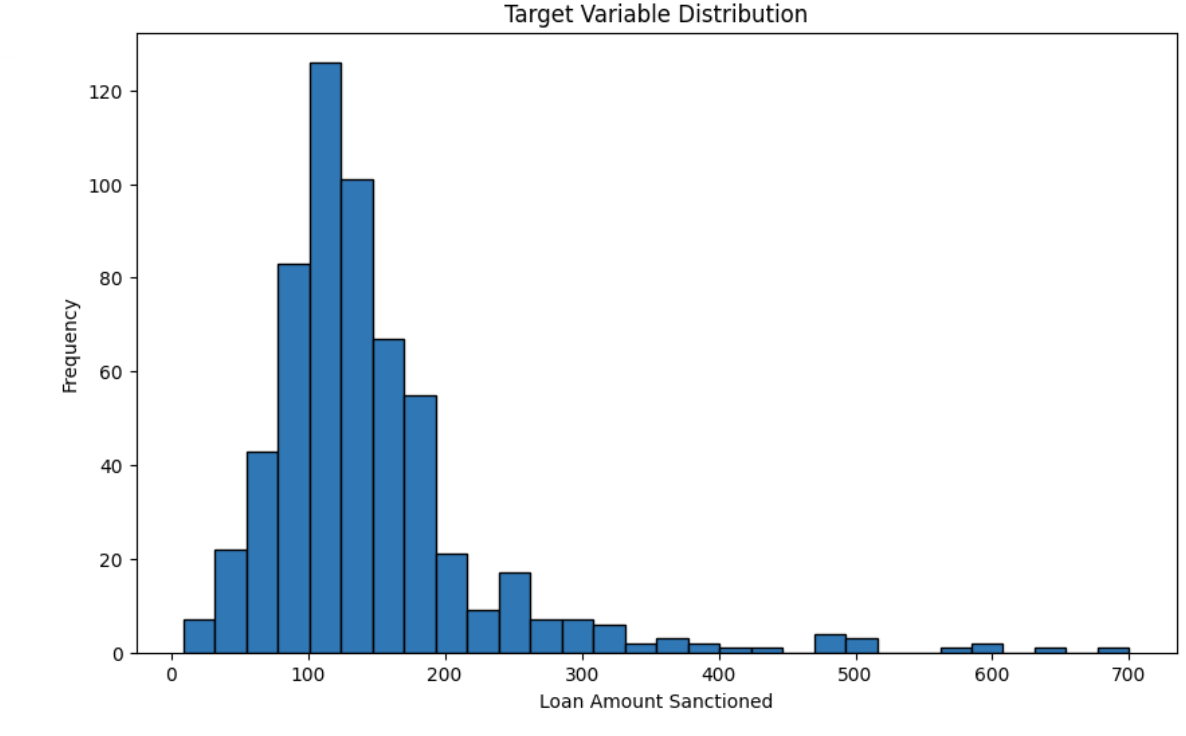
\includegraphics[width=0.75\linewidth]{figs/Target_variable_distribution.png}
}{
    \fbox{\parbox[c][5cm][c]{0.75\linewidth}{\centering
    Insert the exported Colab figure here:\\
    \texttt{target\_distribution.png}}}
}
\caption{Distribution of the target variable (sanctioned loan amount).}
\end{figure}

\textbf{Inference:} The target distribution helps identify the spread and concentration of sanctioned loan amounts. A histogram is useful for identifying whether the target is approximately symmetric or whether it contains skewness or extreme observations. The distribution also provides an initial understanding of the difficulty of the regression task. The model evaluation results indicate that the target contains variation that is only partially explained by the available predictors.

\subsection{Numerical Feature Distributions}

Histograms were generated for the numerical features.

\begin{figure}[H]
\centering
\IfFileExists{figs/numerical_feature_1.png}{
    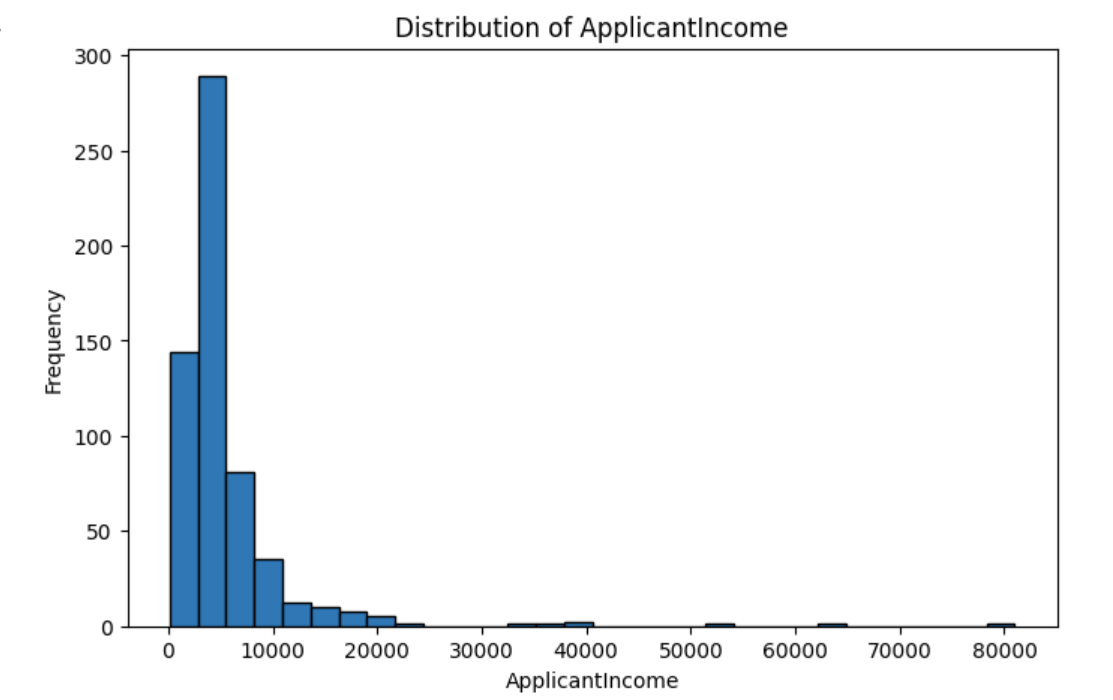
\includegraphics[width=0.8\linewidth]{figs/numerical_feature_1.png}
}{
    \fbox{\parbox[c][5cm][c]{0.8\linewidth}{\centering
    Insert the numerical feature distribution figures here.}}
}
\caption{Distributions of numerical input features.}
\end{figure}

\begin{figure}[H]
\centering
\IfFileExists{figs/numerical_feature_2.png}{
    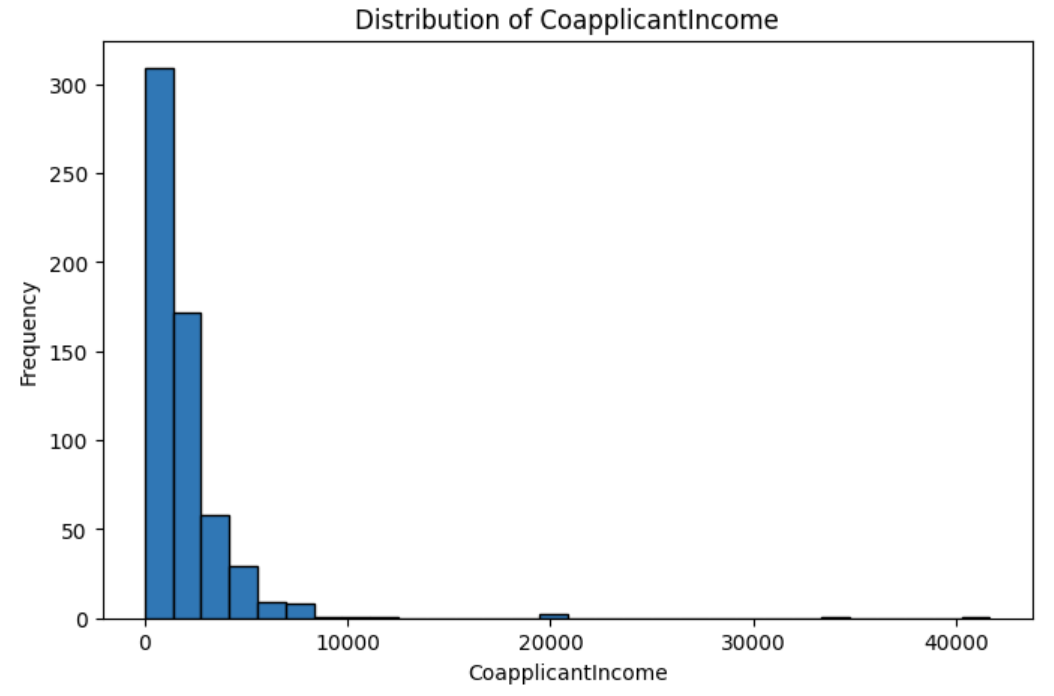
\includegraphics[width=0.8\linewidth]{figs/numerical_feature_2.png}
}{
    \fbox{\parbox[c][5cm][c]{0.8\linewidth}{\centering
    Insert the numerical feature distribution figures here.}}
}
\caption{Distributions of numerical input features.}
\end{figure}

\begin{figure}[H]
\centering
\IfFileExists{figs/numerical_feature_3.png}{
    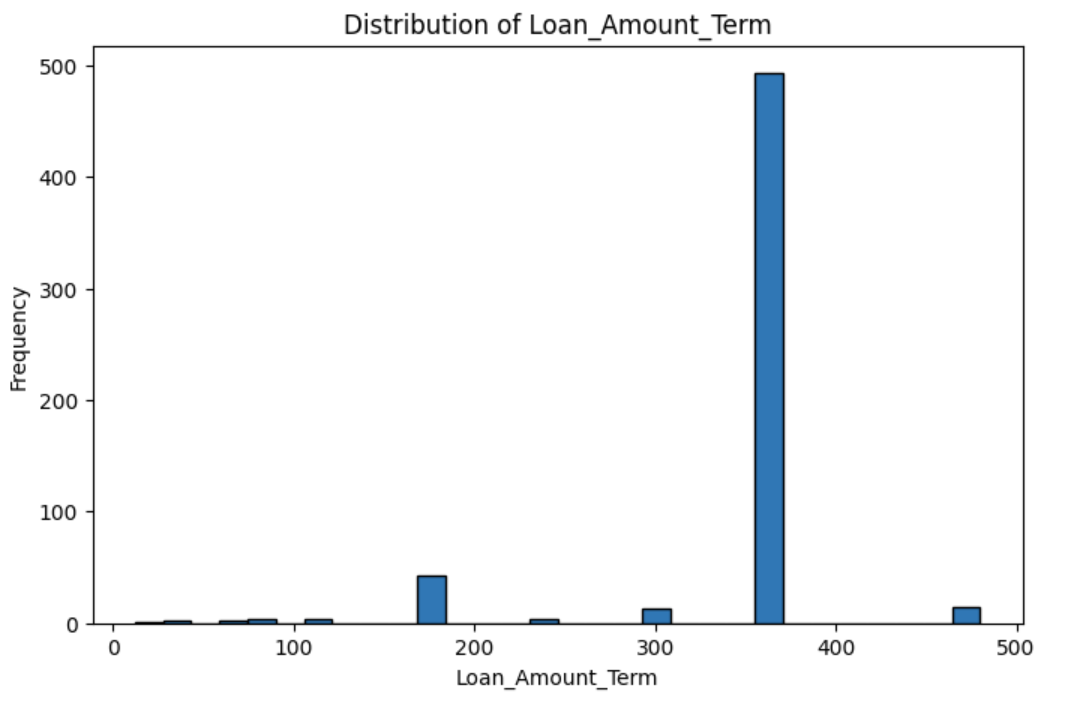
\includegraphics[width=0.8\linewidth]{figs/numerical_feature_3.png}
}{
    \fbox{\parbox[c][5cm][c]{0.8\linewidth}{\centering
    Insert the numerical feature distribution figures here.}}
}
\caption{Distributions of numerical input features.}
\end{figure}

\begin{figure}[H]
\centering
\IfFileExists{figs/numerical_feature_4.png}{
    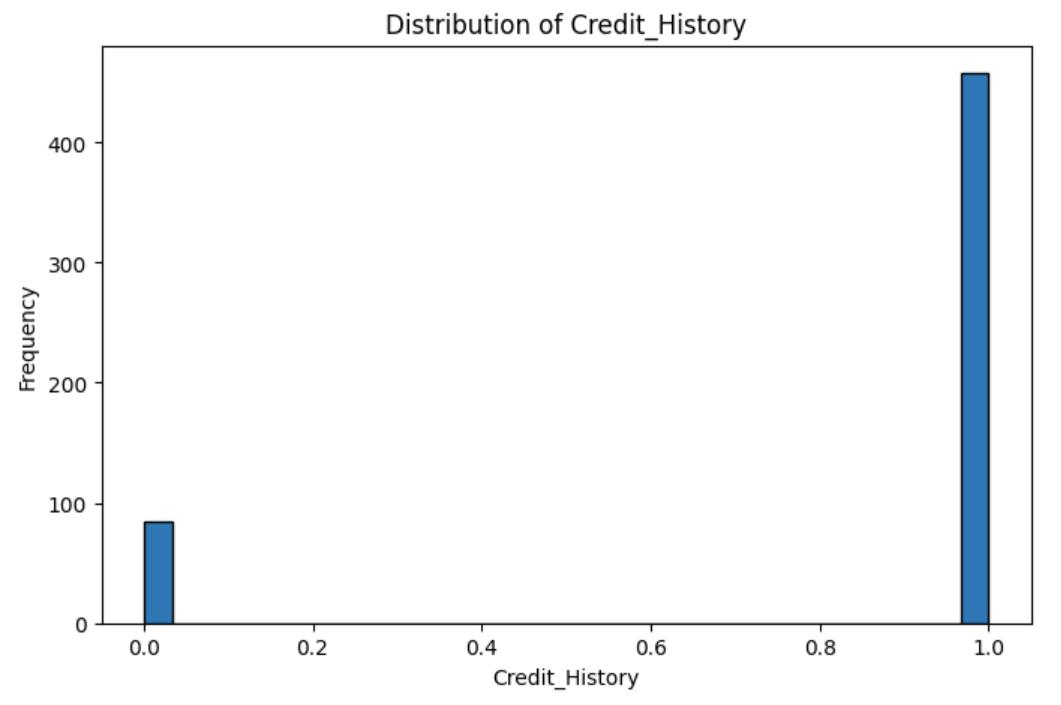
\includegraphics[width=0.8\linewidth]{figs/numerical_feature_4.png}
}{
    \fbox{\parbox[c][5cm][c]{0.8\linewidth}{\centering
    Insert the numerical feature distribution figures here.}}
}
\caption{Distributions of numerical input features.}
\end{figure}
\textbf{Inference:} The numerical-feature distributions show the range and frequency of values for the input variables. Such plots are useful for detecting skewed variables and unusually concentrated observations. These observations motivate the use of median imputation and standardization in the preprocessing pipeline. Standardization is particularly important for regularized regression because the penalty should not be dominated by variables with larger numerical scales.

\subsection{Feature versus Target Analysis}

Scatter plots were generated between selected numerical features and the target variable.

\begin{figure}[H]
\centering
\IfFileExists{figs/target_feature_1.png}{
    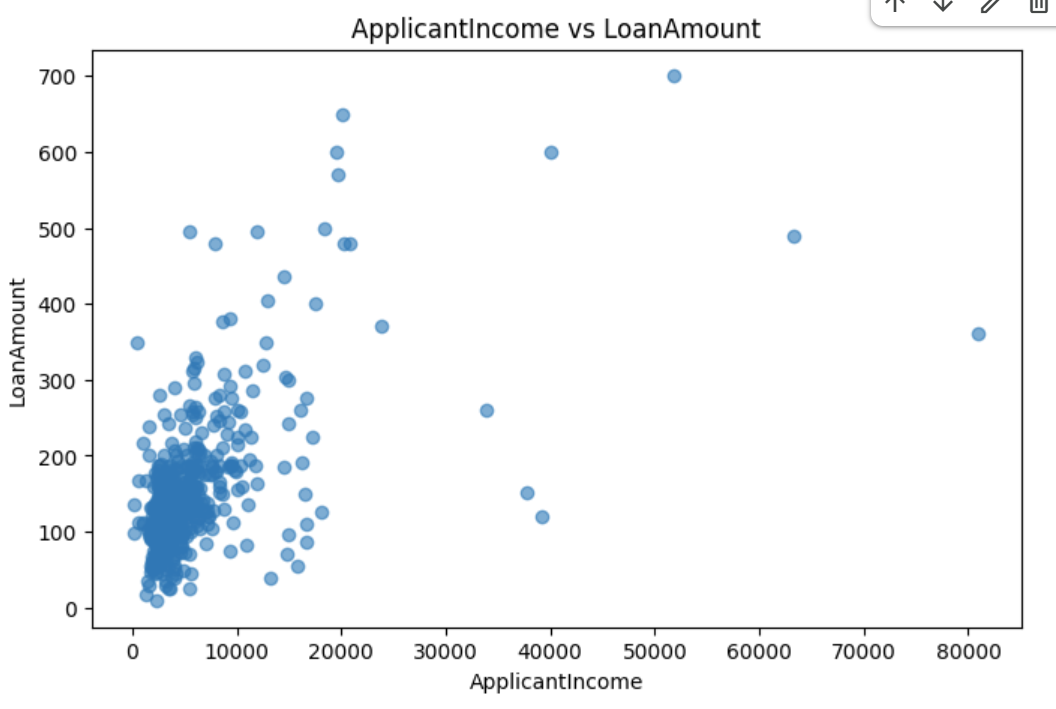
\includegraphics[width=0.8\linewidth]{figs/target_feature_1.png}
}{
    \fbox{\parbox[c][5cm][c]{0.8\linewidth}{\centering
    Insert the feature-versus-target figures here.}}
}
\caption{Relationships between selected numerical features and the sanctioned loan amount.}
\end{figure}

\begin{figure}[H]
\centering
\IfFileExists{figs/target_feature_2.png}{
    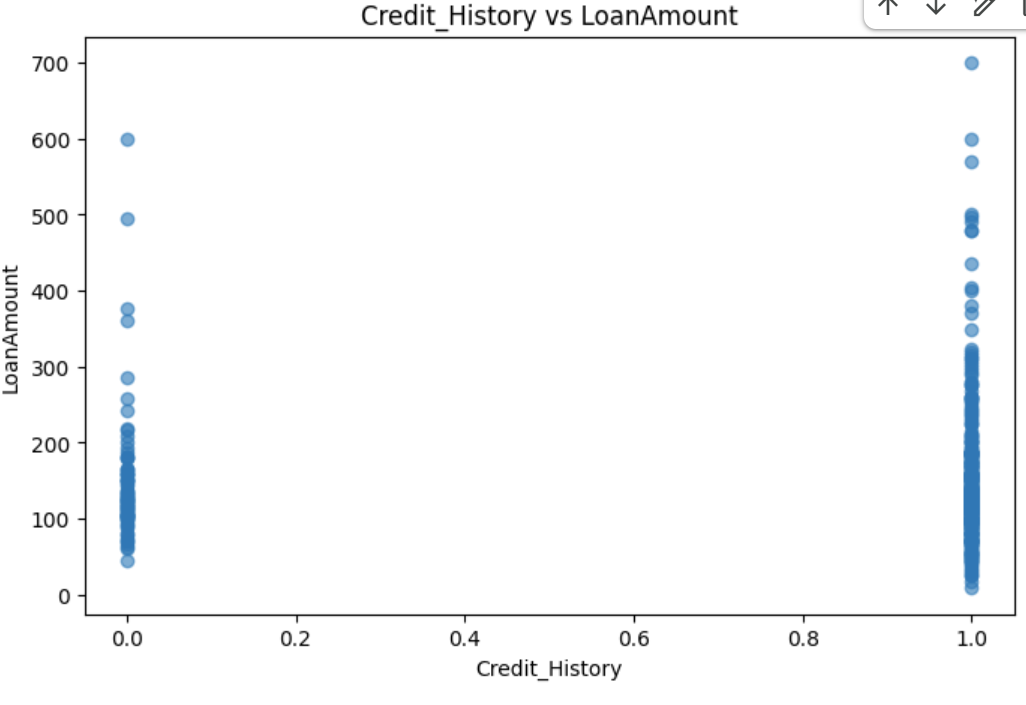
\includegraphics[width=0.8\linewidth]{figs/target_feature_2.png}
}{
    \fbox{\parbox[c][5cm][c]{0.8\linewidth}{\centering
    Insert the feature-versus-target figures here.}}
}
\caption{Relationships between selected numerical features and the sanctioned loan amount.}
\end{figure}

\begin{figure}[H]
\centering
\IfFileExists{figs/target_feature_3.png}{
    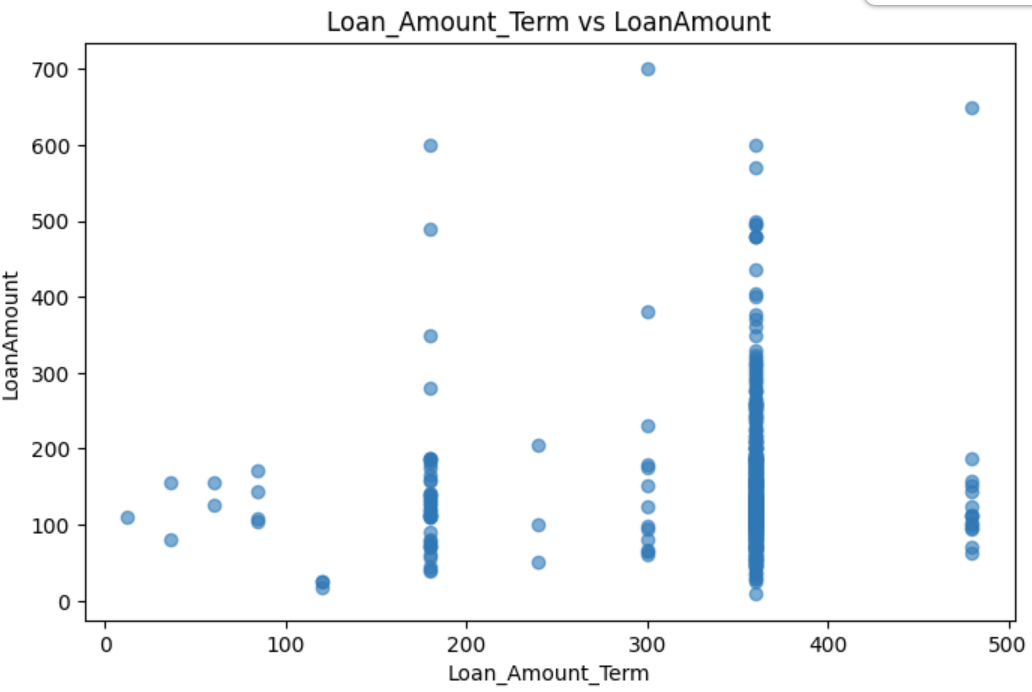
\includegraphics[width=0.8\linewidth]{figs/target_feature_3.png}
}{
    \fbox{\parbox[c][5cm][c]{0.8\linewidth}{\centering
    Insert the feature-versus-target figures here.}}
}
\caption{Relationships between selected numerical features and the sanctioned loan amount.}
\end{figure}

\begin{figure}[H]
\centering
\IfFileExists{figs/target_feature_4.png}{
    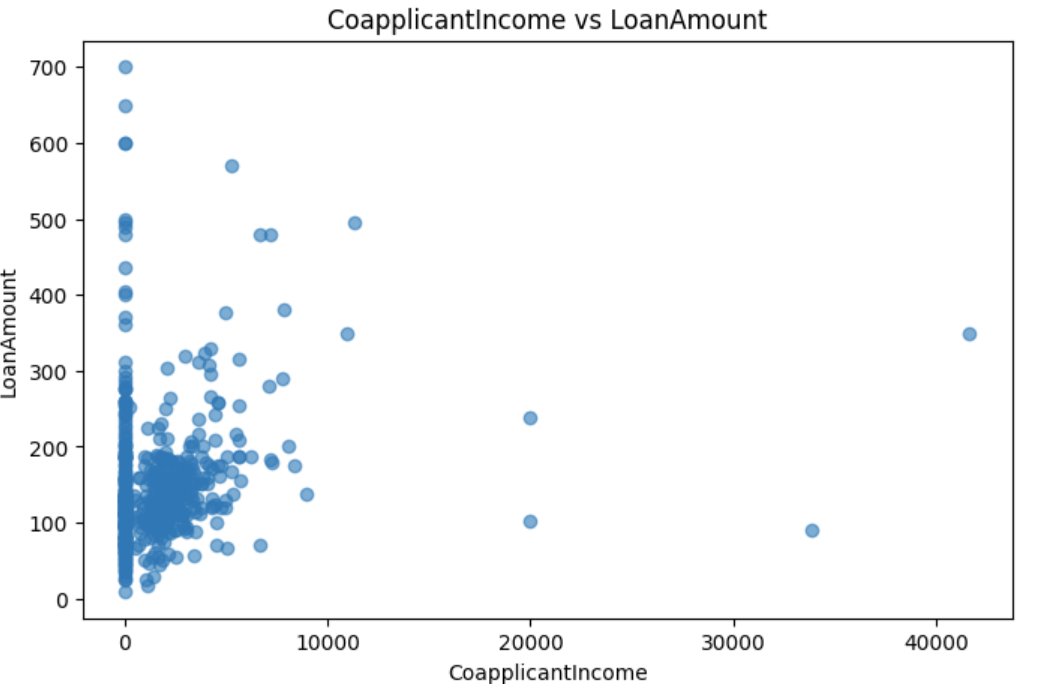
\includegraphics[width=0.8\linewidth]{figs/target_feature_4.png}
}{
    \fbox{\parbox[c][5cm][c]{0.8\linewidth}{\centering
    Insert the feature-versus-target figures here.}}
}
\caption{Relationships between selected numerical features and the sanctioned loan amount.}
\end{figure}

\textbf{Inference:} Feature-versus-target plots provide a visual indication of the relationship between individual predictors and the continuous target. The plots can reveal whether relationships are approximately linear, weak, dispersed, or affected by outliers. Because the regression models use several features simultaneously, a weak individual relationship does not necessarily mean that the feature is useless in the multivariable model.

\subsection{Missing Value Analysis}

Missing values were inspected in the training data. Instead of removing observations indiscriminately, missing numerical values were replaced using the median and missing categorical values were replaced using the most frequent category. The imputation operations were incorporated into the model pipeline so that preprocessing was learned from the training data.

\textbf{Inference:} Imputation prevents loss of observations and allows the regression algorithms to receive complete numerical matrices. Performing imputation inside the pipeline also prevents information from the test set from being used during model fitting.

% ============================================================
\section{Data Preprocessing}
% ============================================================

The preprocessing pipeline was designed separately for numerical and categorical variables.

\subsection{Numerical Feature Processing}

Numerical features were processed using two steps:

\begin{enumerate}
    \item Missing values were replaced with the median of the corresponding training feature.
    \item Numerical variables were standardized using StandardScaler.
\end{enumerate}

Standardization transforms a feature $x$ according to:

\[
z = \frac{x-\mu}{\sigma}
\]

where $\mu$ is the training-set mean and $\sigma$ is the training-set standard deviation.

Scaling is particularly important for Ridge, Lasso, and Elastic Net because their regularization penalties depend on coefficient magnitude.

\subsection{Categorical Feature Processing}

Categorical variables were processed using:

\begin{enumerate}
    \item Most-frequent imputation for missing categorical values.
    \item One-hot encoding to convert categorical variables into numerical indicator variables.
\end{enumerate}

One-hot encoding allows regression algorithms to use categorical information without imposing an artificial numerical ordering on the categories.

\subsection{Train-Test Handling}

The dataset was already divided into separate training and testing CSV files. Therefore, no additional \texttt{train\_test\_split()} operation was used.

The training dataset was used for:

\begin{itemize}
    \item preprocessing fitting,
    \item model training,
    \item five-fold cross-validation,
    \item hyperparameter tuning.
\end{itemize}

The testing dataset was kept for final performance evaluation.

This separation is important because the test set should represent unseen observations when reporting the final model performance.

% ============================================================
\section{Machine Learning Algorithm}
% ============================================================

\subsection{Linear Regression}

Linear Regression models the target as a linear combination of the input features:

\[
\hat{y} = \beta_0 + \beta_1x_1+\beta_2x_2+\cdots+\beta_px_p
\]

The coefficients are estimated by minimizing the residual sum of squares:

\[
\min_{\beta}
\sum_{i=1}^{n}(y_i-\hat{y}_i)^2
\]

Linear Regression was used as the baseline model.

\textbf{Advantages:}

\begin{itemize}
    \item Simple and interpretable.
    \item Computationally efficient.
    \item Provides a useful baseline for comparing regularized models.
\end{itemize}

\textbf{Limitations:}

\begin{itemize}
    \item Can be sensitive to multicollinearity.
    \item Can have high variance when many correlated features are present.
    \item Does not explicitly control model complexity.
\end{itemize}

\subsection{Ridge Regression}

Ridge Regression adds an L2 penalty to the ordinary least-squares objective:

\[
\min_{\beta}
\left[
\sum_{i=1}^{n}(y_i-\hat{y}_i)^2
+
\alpha\sum_{j=1}^{p}\beta_j^2
\right]
\]

The parameter $\alpha$ controls the strength of regularization.

A larger $\alpha$ produces stronger coefficient shrinkage. In this experiment, the best Ridge value was $\alpha=100$.

\textbf{Advantages:}

\begin{itemize}
    \item Reduces coefficient magnitude.
    \item Helps control variance.
    \item Can improve generalization in the presence of correlated predictors.
\end{itemize}

\textbf{Limitation:} Ridge normally does not force coefficients exactly to zero, so it does not provide the same direct feature-selection effect as Lasso.

\subsection{Lasso Regression}

Lasso uses an L1 penalty:

\[
\min_{\beta}
\left[
\sum_{i=1}^{n}(y_i-\hat{y}_i)^2
+
\alpha\sum_{j=1}^{p}|\beta_j|
\right]
\]

The L1 penalty can force some coefficients exactly to zero.

The best value obtained through Grid Search was:

\[
\alpha=1
\]

Lasso produced 602 zero coefficients out of 611 transformed features, corresponding to approximately:

\[
\frac{602}{611}\times100 = 98.53\%
\]

zero coefficients.

\textbf{Advantages:}

\begin{itemize}
    \item Performs regularization.
    \item Performs implicit feature selection.
    \item Produces sparse models.
\end{itemize}

\textbf{Limitation:} Excessive sparsity can remove potentially useful predictors and may increase bias.

\subsection{Elastic Net Regression}

Elastic Net combines L1 and L2 regularization:

\[
\min_{\beta}
\left[
\sum_{i=1}^{n}(y_i-\hat{y}_i)^2
+
\alpha
\left(
\rho\sum_{j=1}^{p}|\beta_j|
+
(1-\rho)\sum_{j=1}^{p}\beta_j^2
\right)
\right]
\]

where $\alpha$ controls the overall regularization strength and $\rho$ (implemented as \texttt{l1\_ratio}) controls the mixture of L1 and L2 penalties.

The best configuration was:

\[
\alpha=1,\qquad l1\_ratio=0.8
\]

Elastic Net therefore provided a combination of coefficient shrinkage and sparsity.

% ============================================================
\section{Experimental Setup}
% ============================================================

\begin{tabular}{ll}
\toprule
Python Version & Google Colab Python environment \\
Scikit-Learn & Scikit-learn library \\
IDE & Google Colab \\
Operating System & Cloud-based Linux environment \\
Hardware & Google Colab runtime \\
Cross-validation & 5-fold K-Fold CV \\
Random State & 42 \\
\bottomrule
\end{tabular}

The exact Python and Scikit-learn version numbers were not recorded in the supplied experiment output. They should be inserted from the Colab environment if required.

% ============================================================
\section{Hyperparameter Selection}
% ============================================================

Five-fold cross-validation and Grid Search were used for selecting regularization parameters.

\begin{table}[H]
\centering
\caption{Hyperparameter search spaces}
\begin{tabular}{lll}
\toprule
\textbf{Model} & \textbf{Parameter} & \textbf{Search Values} \\
\midrule
Ridge & $\alpha$ & 0.01, 0.1, 1, 10, 100 \\
Lasso & $\alpha$ & 0.001, 0.01, 0.1, 1, 10 \\
Elastic Net & $\alpha$ & 0.01, 0.1, 1, 10 \\
Elastic Net & l1\_ratio & 0.2, 0.5, 0.8 \\
\bottomrule
\end{tabular}
\end{table}

\begin{table}[H]
\centering
\caption{Best hyperparameters obtained from Grid Search}
\begin{tabular}{lcc}
\toprule
\textbf{Model} & \textbf{Best Parameters} & \textbf{Best CV $R^2$} \\
\midrule
Ridge & $\alpha=100$ & 0.296446 \\
Lasso & $\alpha=1$ & 0.269309 \\
Elastic Net & $\alpha=1,\ l1\_ratio=0.8$ & 0.291913 \\
\bottomrule
\end{tabular}
\end{table}

The best cross-validation score among the tuned models was obtained by Ridge Regression with $R^2=0.296446$. However, the final model selection was based on the performance on the held-out test set, where Elastic Net achieved the highest $R^2$.

% ============================================================
\section{Results}
% ============================================================

\subsection{Five-Fold Cross-Validation Results}

\begin{table}[H]
\centering
\caption{Five-fold cross-validation performance}
\begin{tabular}{lrrrr}
\toprule
\textbf{Model} & \textbf{MAE} & \textbf{MSE} & \textbf{RMSE} & \textbf{$R^2$} \\
\midrule
Linear Regression & 42.7399 & 5362.2118 & 73.2271 & 0.2629 \\
Ridge Regression & 43.3919 & 5026.3732 & 70.8969 & 0.2964 \\
Lasso Regression & 42.5940 & 5323.2378 & 72.9605 & 0.2693 \\
Elastic Net & 43.5942 & 5061.0426 & 71.1410 & 0.2919 \\
\bottomrule
\end{tabular}
\end{table}

\subsection{Final Test-Set Results}

The final evaluation was performed using the supplied testing dataset containing 362 observations.

\begin{table}[H]
\centering
\caption{Final test-set performance}
\begin{tabular}{lrrrrr}
\toprule
\textbf{Model} & \textbf{MAE} & \textbf{MSE} & \textbf{RMSE} & \textbf{$R^2$} & \textbf{Time (s)} \\
\midrule
Linear Regression & 36.0467 & 2728.8873 & 52.2388 & 0.2734 & 0.2250 \\
Ridge Regression & 35.7577 & 2606.4552 & 51.0535 & 0.3060 & 5.4762 \\
Lasso Regression & 35.4400 & 2660.1341 & 51.5765 & 0.2917 & 8.6063 \\
Elastic Net & 35.7653 & 2587.4734 & 50.8672 & \textbf{0.3110} & 2.5264 \\
\bottomrule
\end{tabular}
\end{table}

\subsection{Interpretation of Results}

Elastic Net Regression achieved the highest final test-set $R^2$ score of 0.3110. It also achieved the lowest MSE of 2587.4734 and the lowest RMSE of 50.8672. Therefore, Elastic Net was selected as the best overall model.

Lasso Regression achieved the lowest MAE of 35.4400. This means that Lasso produced the smallest average absolute prediction error. However, its $R^2$ score was 0.2917, lower than the 0.3110 obtained by Elastic Net.

Ridge Regression achieved the second-highest test $R^2$ score of 0.3060. It also performed better than Linear Regression on MSE, RMSE, and $R^2$, demonstrating the benefit of regularization.

The test-set results show that regularization improved generalization compared with the baseline Linear Regression model.

% ============================================================
\section{Result Visualization}
% ============================================================

\subsection{Predicted versus Actual Values}

\begin{figure}[H]
\centering
\IfFileExists{figs/predicted_vs_actual_1.png}{
    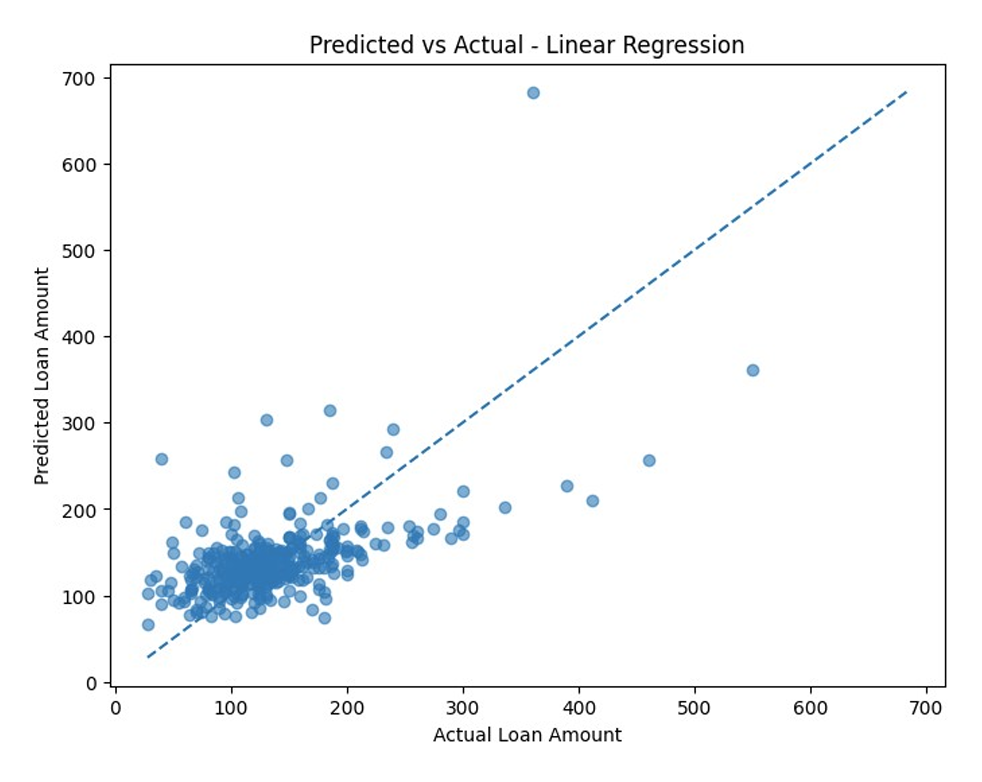
\includegraphics[width=0.78\linewidth]{figs/predicted_vs_actual_1.png}
}{
    \fbox{\parbox[c][5cm][c]{0.78\linewidth}{\centering
    Insert the Predicted vs Actual graph exported from Colab.}}
}
\caption{Predicted versus actual loan amounts for the regression models.}
\end{figure}

\begin{figure}[H]
\centering
\IfFileExists{figs/predicted_vs_actual_2.png}{
    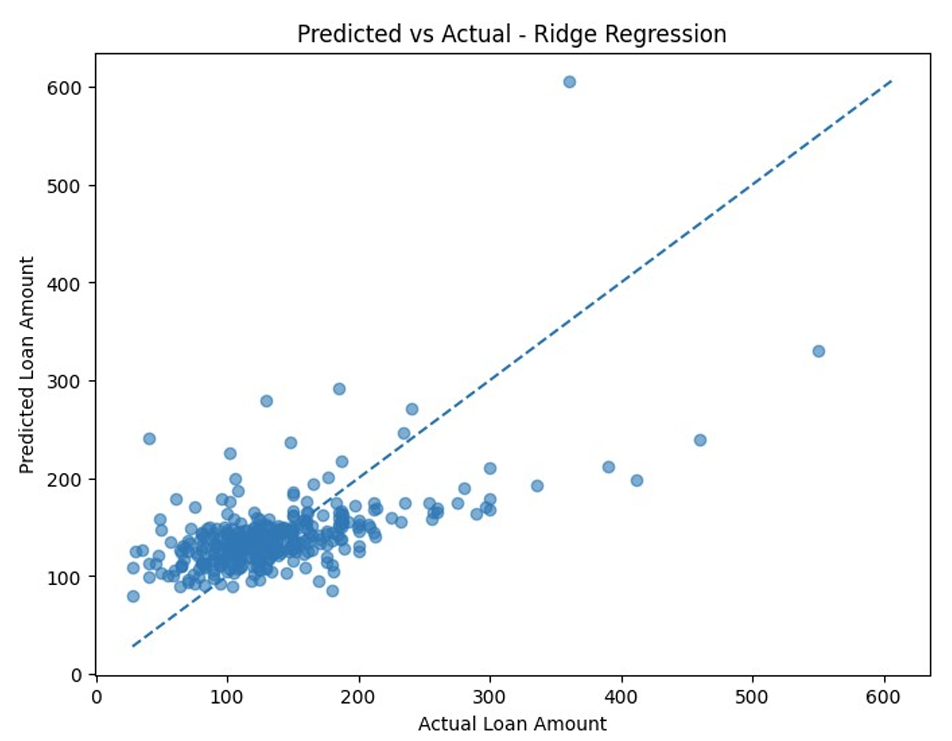
\includegraphics[width=0.78\linewidth]{figs/predicted_vs_actual_2.png}
}{
    \fbox{\parbox[c][5cm][c]{0.78\linewidth}{\centering
    Insert the Predicted vs Actual graph exported from Colab.}}
}
\caption{Predicted versus actual loan amounts for the regression models.}
\end{figure}

\begin{figure}[H]
\centering
\IfFileExists{figs/predicted_vs_actual_3.png}{
    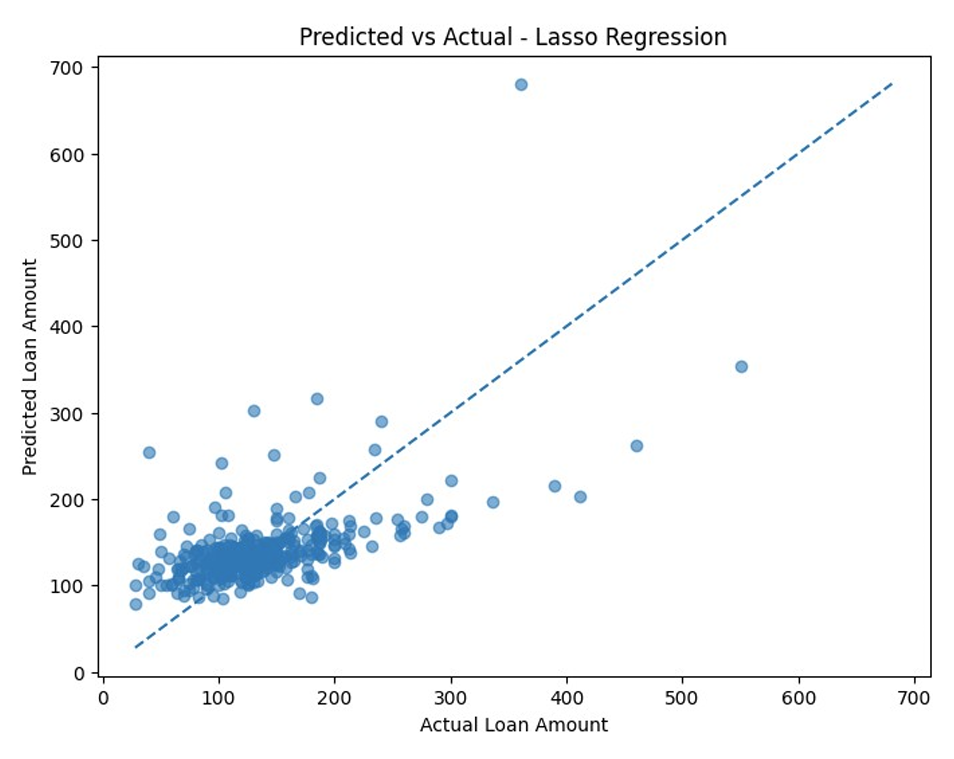
\includegraphics[width=0.78\linewidth]{figs/predicted_vs_actual_3.png}
}{
    \fbox{\parbox[c][5cm][c]{0.78\linewidth}{\centering
    Insert the Predicted vs Actual graph exported from Colab.}}
}
\caption{Predicted versus actual loan amounts for the regression models.}
\end{figure}

\begin{figure}[H]
\centering
\IfFileExists{figs/predicted_vs_actual_4.png}{
    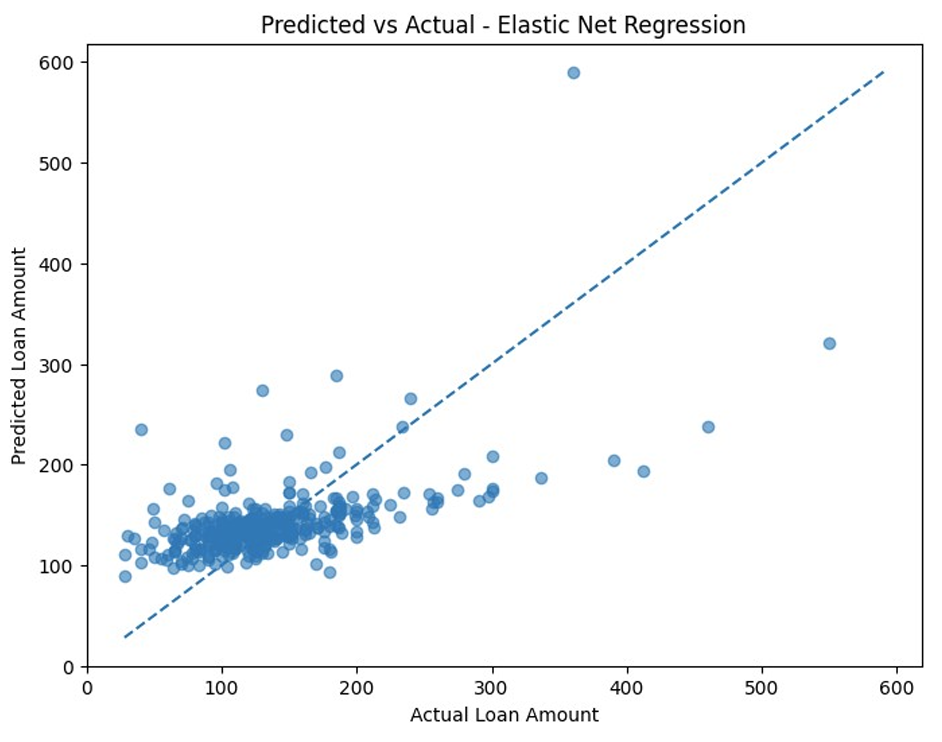
\includegraphics[width=0.78\linewidth]{figs/predicted_vs_actual_4.png}
}{
    \fbox{\parbox[c][5cm][c]{0.78\linewidth}{\centering
    Insert the Predicted vs Actual graph exported from Colab.}}
}
\caption{Predicted versus actual loan amounts for the regression models.}
\end{figure}

\textbf{Inference:} The predicted-versus-actual plot is used to evaluate how closely model predictions follow the actual target values. Points close to the diagonal reference line indicate more accurate predictions. The dispersion of points around the line indicates prediction error. Elastic Net produced the strongest overall test performance according to $R^2$, MSE, and RMSE.

\subsection{Residual Analysis}

\begin{figure}[H]
\centering
\IfFileExists{figs/residual_plot_1.png}{
    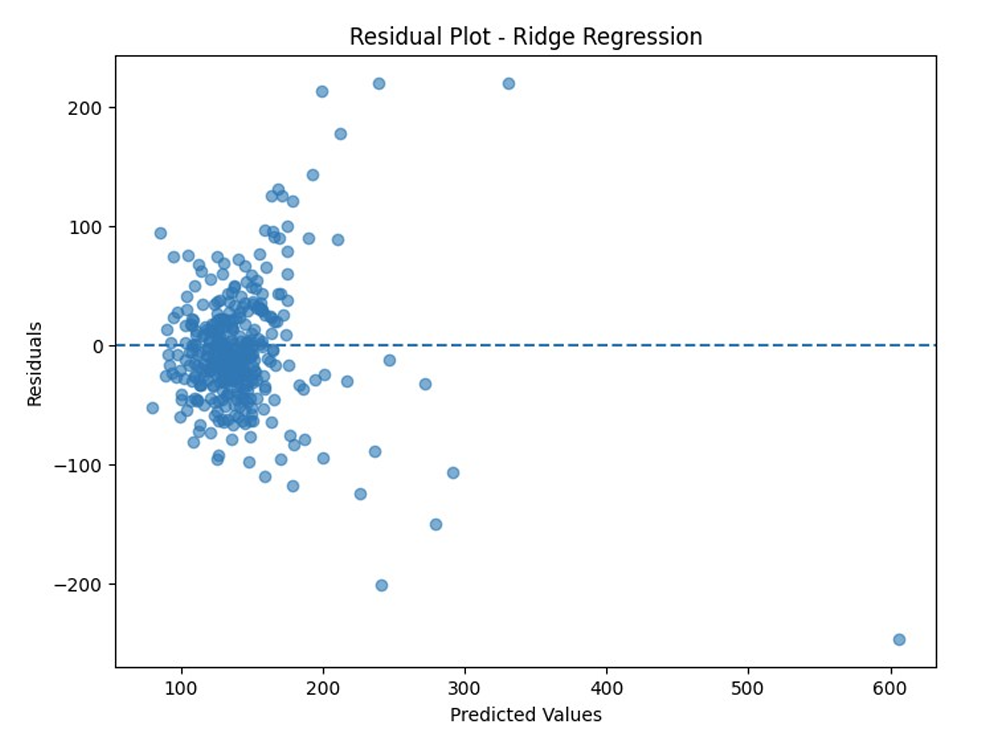
\includegraphics[width=0.78\linewidth]{figs/residual_plot_1.png}
}{
    \fbox{\parbox[c][5cm][c]{0.78\linewidth}{\centering
    Insert the residual plots exported from Colab.}}
}
\caption{Residual plots for the regression models.}
\end{figure}

\begin{figure}[H]
\centering
\IfFileExists{figs/residual_plot_2.png}{
    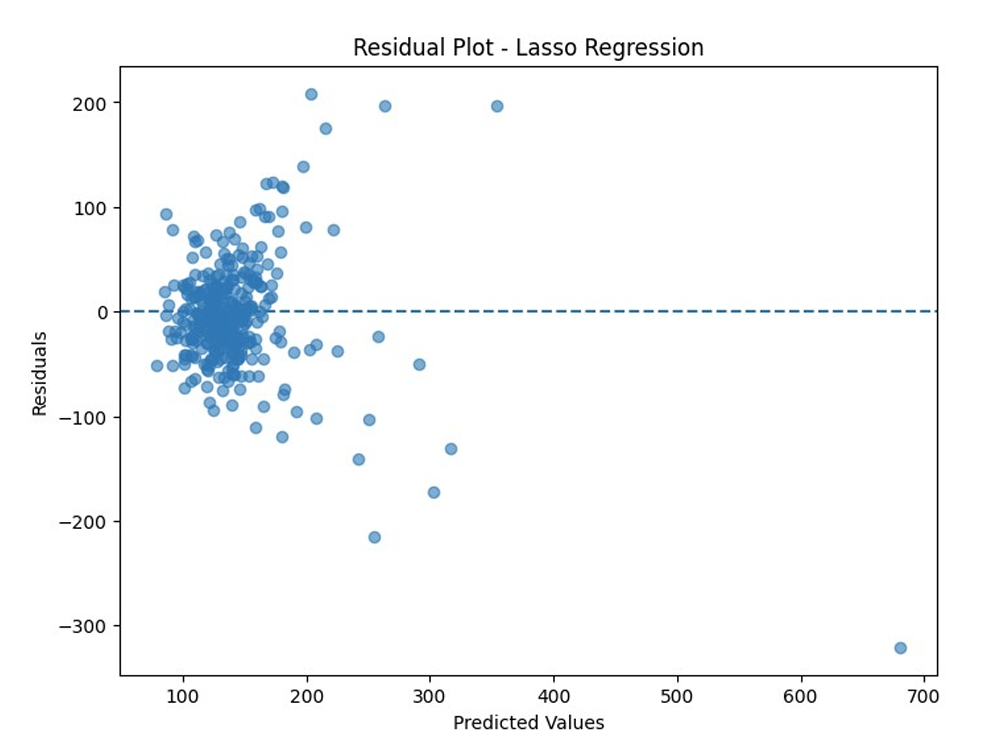
\includegraphics[width=0.78\linewidth]{figs/residual_plot_2.png}
}{
    \fbox{\parbox[c][5cm][c]{0.78\linewidth}{\centering
    Insert the residual plots exported from Colab.}}
}
\caption{Residual plots for the regression models.}
\end{figure}

\begin{figure}[H]
\centering
\IfFileExists{figs/residual_plot_3.png}{
    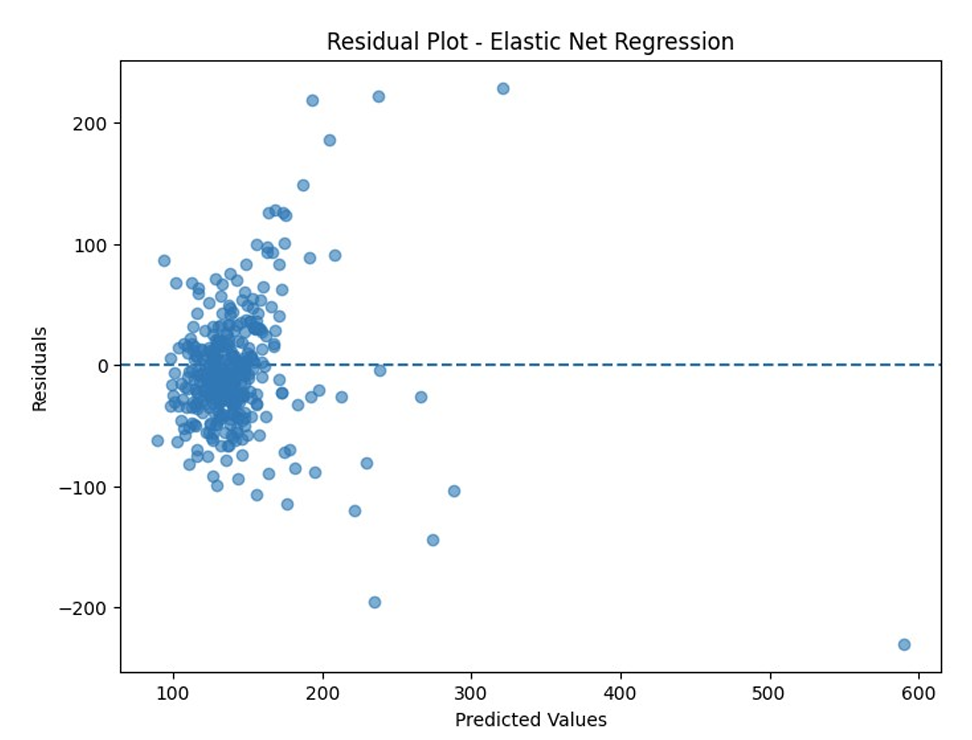
\includegraphics[width=0.78\linewidth]{figs/residual_plot_3.png}
}{
    \fbox{\parbox[c][5cm][c]{0.78\linewidth}{\centering
    Insert the residual plots exported from Colab.}}
}
\caption{Residual plots for the regression models.}
\end{figure}

\textbf{Inference:} Residual plots show the difference between observed and predicted values. A desirable residual pattern is approximately centered around zero without a strong systematic structure. Systematic patterns can indicate model inadequacy or non-linearity. Residual analysis therefore provides a complementary assessment beyond numerical metrics.

\subsection{Training Error versus Test Error}

\begin{figure}[H]
\centering
\IfFileExists{figs/train_vs_test.png}{
    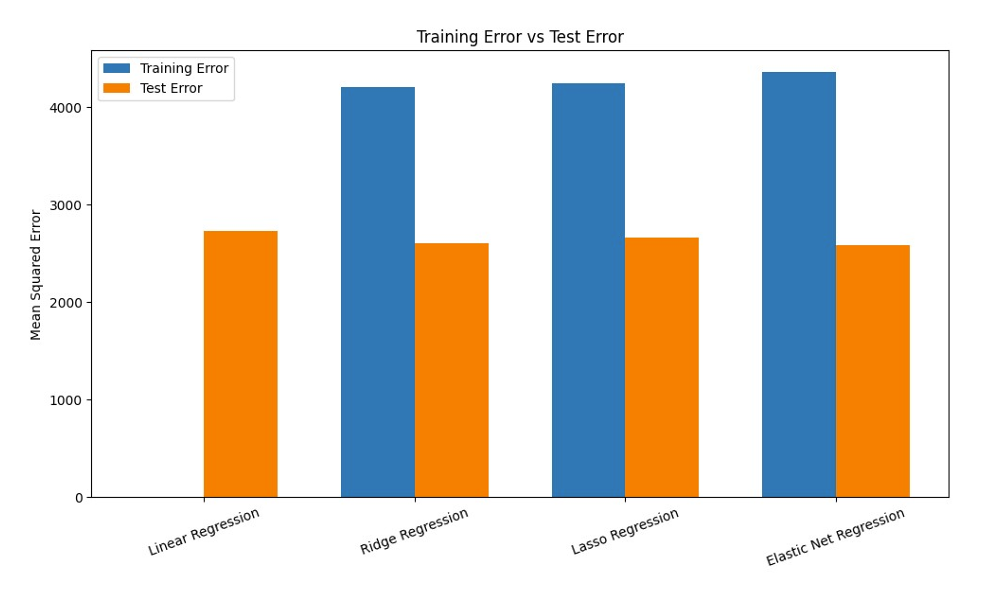
\includegraphics[width=0.78\linewidth]{figs/train_vs_test.png}
}{
    \fbox{\parbox[c][5cm][c]{0.78\linewidth}{\centering
    Insert the Training Error vs Test Error graph exported from Colab.}}
}
\caption{Comparison of training and test mean squared error.}
\end{figure}

\textbf{Inference:} Linear Regression obtained an extremely small training MSE but a larger test MSE, showing that it fits the training observations very closely. The regularized models have larger training errors but lower test errors. This pattern is consistent with regularization reducing variance and improving generalization.

\subsection{$R^2$ Score Comparison}

\begin{figure}[H]
\centering
\IfFileExists{figs/r2_comparsion.png}{
    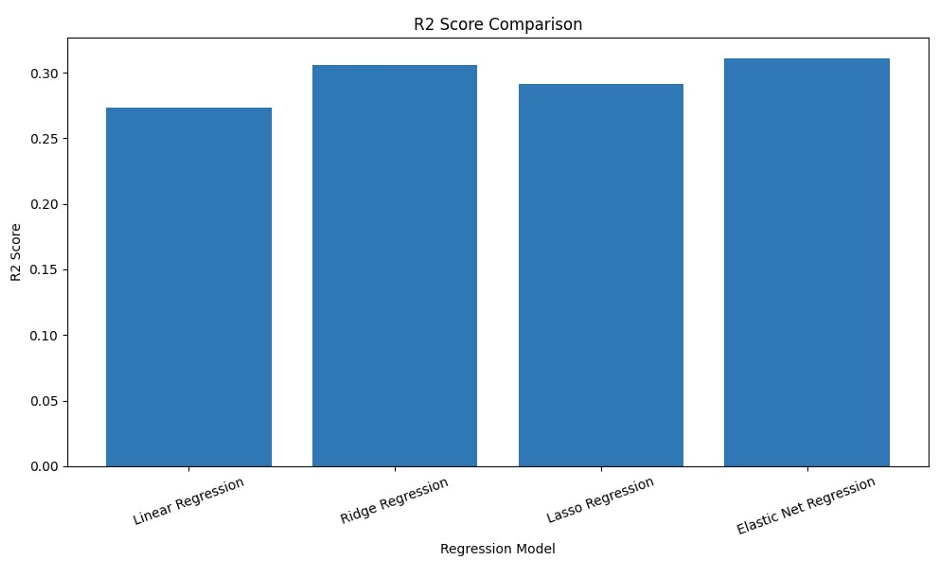
\includegraphics[width=0.78\linewidth]{figs/r2_comparsion.png}
}{
    \fbox{\parbox[c][5cm][c]{0.78\linewidth}{\centering
    Insert the R-squared comparison graph exported from Colab.}}
}
\caption{$R^2$ score comparison of the regression models.}
\end{figure}

\textbf{Inference:} Elastic Net achieved the highest test $R^2$ score of 0.3110, followed by Ridge with 0.3060. Lasso achieved 0.2917, while Linear Regression achieved 0.2734. The results indicate that regularization improves the proportion of target variation explained by the model on unseen data.

\subsection{Coefficient Comparison}

\begin{figure}[H]
\centering
\IfFileExists{figs/coefficient_comparsion.png}{
    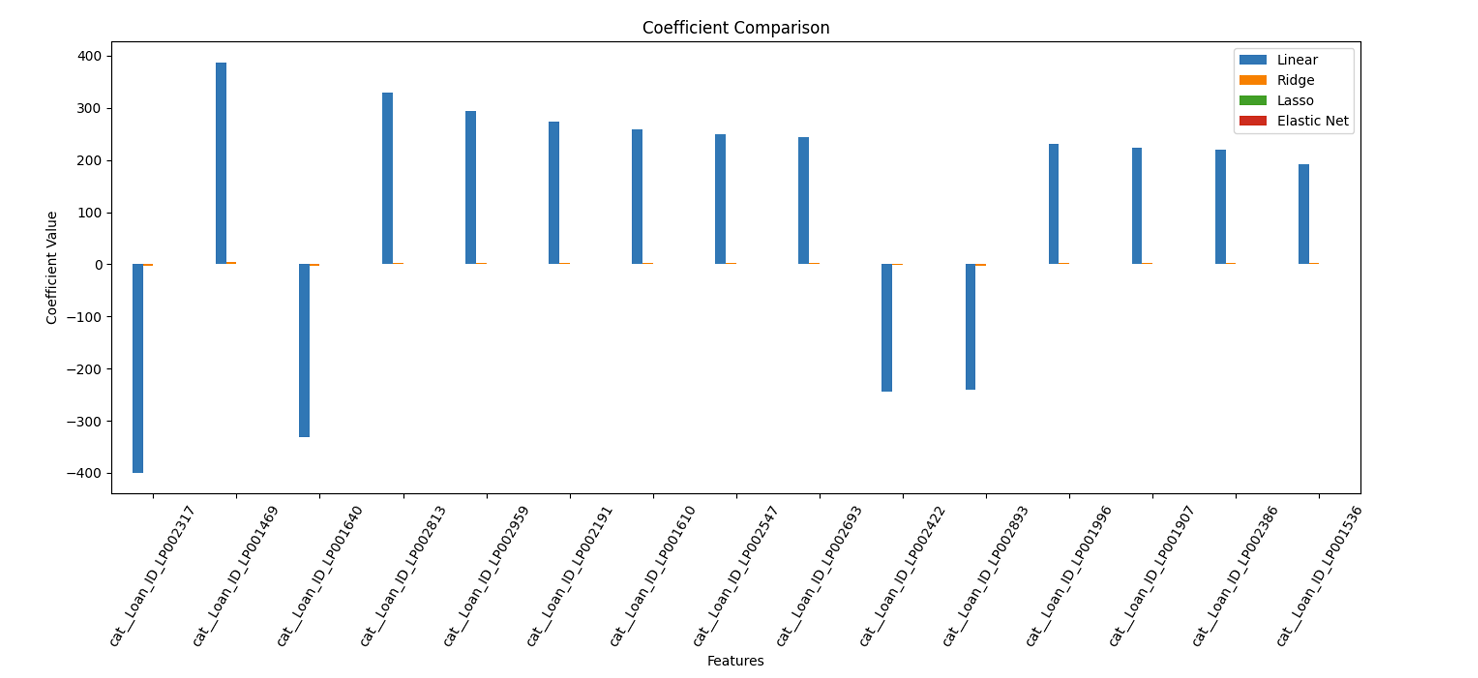
\includegraphics[width=0.78\linewidth]{figs/coefficient_comparsion.png}
}{
    \fbox{\parbox[c][5cm][c]{0.78\linewidth}{\centering
    Insert the coefficient comparison graph exported from Colab.}}
}
\caption{Comparison of regression coefficients across models.}
\end{figure}

\textbf{Inference:} The coefficient comparison demonstrates the effect of regularization on model parameters. Ridge shrinks coefficients toward zero, while Lasso can set coefficients exactly to zero. Elastic Net combines both effects. This analysis helps explain how regularization controls model complexity.

% ============================================================
\section{Discussion}
% ============================================================

\subsection{Model Comparison}

The four models provide different approaches to controlling model complexity.

\textbf{Linear Regression} serves as the baseline. It obtained a test $R^2$ of 0.2734. Its very low training MSE indicates that it can fit the training data extremely closely, but its test performance is weaker than the regularized models.

\textbf{Ridge Regression} obtained a test $R^2$ of 0.3060. The L2 penalty reduced coefficient magnitude and improved test generalization. Its best regularization strength was $\alpha=100$.

\textbf{Lasso Regression} obtained a test $R^2$ of 0.2917 and the lowest MAE of 35.4400. It also produced a highly sparse model, with 602 of 611 transformed coefficients equal to zero.

\textbf{Elastic Net Regression} achieved the best overall test performance. Its test $R^2$ was 0.3110, while its MSE and RMSE were also the lowest among the four models. Its optimal parameters were $\alpha=1$ and $l1\_ratio=0.8$.

\subsection{Overfitting and Underfitting}

The training and test errors demonstrate why regularization is useful. Linear Regression has a training MSE close to zero, whereas its test MSE is 2728.8873. This large difference indicates that the unregularized model fits the training data very closely and does not generalize as well as the regularized alternatives.

The regularized models accept a higher training error in exchange for better test performance. Ridge, Lasso, and Elastic Net all have lower test MSE than Linear Regression. This indicates that the regularization penalties help reduce variance and improve generalization.

The results do not provide evidence of severe underfitting in the sense of identical poor training and test performance. Instead, the primary observation is that the unregularized model benefits from regularization when evaluated on unseen data.

\subsection{Bias--Variance Trade-off}

Regularization introduces a controlled amount of bias in exchange for a reduction in variance.

Linear Regression has less constraint on its coefficients and can therefore achieve extremely low training error. However, this flexibility can lead to higher variance.

Ridge introduces an L2 penalty and reduces coefficient magnitude. This generally reduces variance while retaining all predictors.

Lasso introduces an L1 penalty and performs feature selection. Its strong sparsity result shows that it removed most transformed coefficients.

Elastic Net combines L1 and L2 penalties. In this experiment, this combination produced the best final test-set performance, suggesting that it provided a favorable balance between bias and variance for this dataset.

\subsection{Feature Sparsity}

Lasso produced 602 zero coefficients out of 611 transformed features. The resulting sparsity was:

\[
98.53\%
\]

This demonstrates that L1 regularization can substantially simplify a model by removing many transformed predictors. However, such high sparsity should be interpreted carefully because removing too many coefficients can also discard useful information.

\subsection{Strengths}

The experiment has several strengths:

\begin{itemize}
    \item Four different regression strategies were compared.
    \item A predefined test set was kept separate from model training.
    \item Five-fold cross-validation was used for model selection.
    \item Grid Search was used for systematic hyperparameter tuning.
    \item Both numerical and categorical features were handled through a unified preprocessing pipeline.
    \item Multiple evaluation metrics were used rather than relying on a single score.
    \item Coefficient behavior and Lasso sparsity were analyzed.
\end{itemize}

\subsection{Limitations}

The models explain only about 27--31\% of the variance in the test target, as indicated by the $R^2$ values. This suggests that the available features do not fully explain variation in sanctioned loan amounts.

Another limitation is that the dataset contains an identifier-type variable, \texttt{Loan\_ID}, which was treated as a categorical feature in the supplied implementation. Identifier variables generally have limited predictive meaning and can create a large number of one-hot encoded columns. The resulting 611 transformed features also contribute to the high dimensionality of the model.

The experiment evaluates linear and regularized linear models. Non-linear relationships may not be captured adequately by these models.

\subsection{Possible Improvements}

Possible improvements include:

\begin{enumerate}
    \item Removing identifier variables such as \texttt{Loan\_ID} if they do not carry meaningful predictive information.
    \item Creating domain-based features such as total household income.
    \item Testing non-linear regression methods for comparison.
    \item Investigating outliers and highly skewed variables.
    \item Using additional feature engineering based on the meaning of the loan application variables.
    \item Performing broader hyperparameter searches if computational resources permit.
\end{enumerate}

% ============================================================
\section{Conclusion}
% ============================================================

This experiment implemented and compared Linear Regression, Ridge Regression, Lasso Regression, and Elastic Net Regression for predicting sanctioned loan amounts.

The preprocessing pipeline handled missing values, encoded categorical variables, and standardized numerical variables. Five-fold cross-validation and Grid Search were used to select regularization parameters for Ridge, Lasso, and Elastic Net.

The final test-set results showed that Elastic Net was the best overall model, achieving an $R^2$ score of \textbf{0.3110}, MSE of \textbf{2587.4734}, and RMSE of \textbf{50.8672}. Ridge was the second-best model based on $R^2$, with a score of 0.3060. Lasso achieved the lowest MAE of 35.4400 and demonstrated strong feature sparsity, with 98.53\% of transformed coefficients reduced to zero.

The experiment therefore demonstrates that regularization can improve generalization compared with ordinary Linear Regression. Elastic Net provided the best overall balance of prediction performance and regularization for the supplied dataset and was selected as the final model.

% ============================================================
\section{References}
% ============================================================

\begin{enumerate}[label={[}\arabic*{]}]
    \item C. M. Bishop, \textit{Pattern Recognition and Machine Learning}. New York, NY, USA: Springer, 2006.

    \item T. Hastie, R. Tibshirani, and J. Friedman, \textit{The Elements of Statistical Learning: Data Mining, Inference, and Prediction}, 2nd ed. New York, NY, USA: Springer, 2009.

    \item Scikit-learn Developers, ``Linear Models,'' Scikit-learn Documentation. [Online]. Available: \url{https://scikit-learn.org/stable/modules/linear_model.html}

    \item Scikit-learn Developers, ``Preprocessing data,'' Scikit-learn Documentation. [Online]. Available: \url{https://scikit-learn.org/stable/modules/preprocessing.html}

    \item Scikit-learn Developers, ``Model selection and evaluation,'' Scikit-learn Documentation. [Online]. Available: \url{https://scikit-learn.org/stable/model_selection.html}

    \item Scikit-learn Developers, ``Metrics and scoring: quantifying the quality of predictions,'' Scikit-learn Documentation. [Online]. Available: \url{https://scikit-learn.org/stable/modules/model_evaluation.html}
\end{enumerate}

% ============================================================
\appendix
\section{Appendix A: Important Experimental Results}

\begin{table}[H]
\centering
\caption{Summary of final model selection}
\begin{tabular}{lr}
\toprule
\textbf{Quantity} & \textbf{Value} \\
\midrule
Best Model & Elastic Net Regression \\
Best Test $R^2$ & 0.3110108 \\
Best Test MSE & 2587.4734 \\
Best Test RMSE & 50.8672 \\
Best Test MAE & 35.7653 \\
Best Elastic Net $\alpha$ & 1 \\
Best Elastic Net $l1\_ratio$ & 0.8 \\
Transformed Features & 611 \\
Lasso Zero Coefficients & 602 \\
Lasso Sparsity & 98.53\% \\
\bottomrule
\end{tabular}
\end{table}

\section{Appendix B: Core Python Implementation}

\begin{lstlisting}
# Separate features and target
X_train = train_df.drop(columns=[target_column])
y_train = train_df[target_column]

X_test = test_df.drop(columns=[target_column])
y_test = test_df[target_column]

# Numerical preprocessing
numeric_transformer = Pipeline(
    steps=[
        ("imputer", SimpleImputer(strategy="median")),
        ("scaler", StandardScaler())
    ]
)

# Categorical preprocessing
categorical_transformer = Pipeline(
    steps=[
        ("imputer",
         SimpleImputer(strategy="most_frequent")),
        ("encoder",
         OneHotEncoder(handle_unknown="ignore",
                       sparse_output=False))
    ]
)

# Combined preprocessing
preprocessor = ColumnTransformer(
    transformers=[
        ("num", numeric_transformer, numeric_features),
        ("cat", categorical_transformer, categorical_features)
    ]
)

# Elastic Net model
elastic_pipeline = Pipeline(
    steps=[
        ("preprocessor", preprocessor),
        ("model", ElasticNet(max_iter=10000))
    ]
)

# Grid Search
elastic_params = {
    "model__alpha": [0.01, 0.1, 1, 10],
    "model__l1_ratio": [0.2, 0.5, 0.8]
}

elastic_grid = GridSearchCV(
    elastic_pipeline,
    elastic_params,
    cv=5,
    scoring="r2",
    n_jobs=-1
)

elastic_grid.fit(X_train, y_train)

# Final predictions
elastic_test_pred = elastic_grid.predict(X_test)
\end{lstlisting}

\end{document}
